%%%%%%%%%%%%%%%%%%%%%%%%%%%%%%%%%%%%
% Slide options
%%%%%%%%%%%%%%%%%%%%%%%%%%%%%%%%%%%%

% Option 1: Slides with solutions

\documentclass[slidestop,compress,mathserif]{beamer}
\usepackage{pgfplots}
\newcommand{\soln}[1]{\textit{#1}}
\newcommand{\solnGr}[1]{#1}

% Option 2: Handouts without solutions

%\documentclass[11pt,containsverbatim,handout]{beamer}
%\usepackage{pgfpages}
%\pgfpagesuselayout{4 on 1}[letterpaper,landscape,border shrink=5mm]
%\newcommand{\soln}[1]{ }
%\newcommand{\solnGr}{ }

%%%%%%%%%%%%%%%%%%%%%%%%%%%%%%%%%%%%
% Style
%%%%%%%%%%%%%%%%%%%%%%%%%%%%%%%%%%%%

%%%%%%%%%%%%%%%%%%%%%%%%%%%%%%%%%%%%%%%%%%%%%%%%%%%%%%%%%%%%%%%%%%%%%%%%
% MA213/214 shared slide style
%
% "Calm & Cool" palette + content-type callout boxes.
% Overhauled (2026) from the original OpenIntro/metropolis style:
%   - all OpenIntro visual branding removed (logo, grid, colors)
%   - a low-key cool palette (see colors below)
%   - tcolorbox callout boxes so students recognize content types
% See common/README.md for the command cheat-sheet.
%%%%%%%%%%%%%%%%%%%%%%%%%%%%%%%%%%%%%%%%%%%%%%%%%%%%%%%%%%%%%%%%%%%%%%%%

\usetheme{metropolis}

%%%%%%%%%%%%%%%%
% Packages
%%%%%%%%%%%%%%%%

\usepackage{geometry}
\usepackage{graphicx}
\usepackage{amssymb}
\usepackage{epstopdf}
\usepackage{amsmath}  	% this permits text in eqnarray among other benefits
\usepackage{url}		% produces hyperlinks
\usepackage{hyperref}	% allows for color usage in tables
\usepackage[english]{babel}
\usepackage[latin1]{inputenc}
\usepackage{colortbl}	% allows for color usage in tables
\usepackage{multirow}	% allows for rows that span multiple rows in tables
\usepackage{color}		% this package has a variety of color options
\usepackage{pgf}
\usepackage{calc}
\usepackage{ulem}
\usepackage{multicol}
\usepackage{textcomp}
\usepackage{txfonts}
\usepackage{listings}
\usepackage{tikz}
\usepackage{array}
\usepackage{wasysym}
\usepackage{fancyvrb}
\usepackage{etoolbox}             % \ifstrempty for optional box subtitles
\usepackage[most]{tcolorbox}      % content-type callout boxes
\tcbuselibrary{listings}          % R-code block (\begin{rblock})
\usepackage{fontawesome5}         % box icons

%%%%%%%%%%%%%%%%
% Remove navigation symbols
%%%%%%%%%%%%%%%%

\setbeamertemplate{navigation symbols}{}

%%%%%%%%%%%%%%%%
% "Calm & Cool" palette
%%%%%%%%%%%%%%%%

% chrome / structure / body
\definecolor{ccSlate}{HTML}{2E3742}   % frametitle bar, structure, section pages (deep neutral slate)
\definecolor{ccInk}{HTML}{2B2B2B}     % body text
\definecolor{ccWash}{HTML}{FCF8F1}    % gentle warm title-slide background wash (complements the cool blues)

% example (blue)
\definecolor{ccBlue}{HTML}{2F6690}
\definecolor{ccBlueBg}{HTML}{EAF1F7}
% interactive activity / discussion (green)
\definecolor{ccGreen}{HTML}{4E8A6B}
\definecolor{ccGreenBg}{HTML}{E9F3EC}
% solution (purple)
\definecolor{ccPurple}{HTML}{6F5499}
\definecolor{ccPurpleBg}{HTML}{EFEAF6}
% worksheet / focused work (terracotta)
\definecolor{ccTerra}{HTML}{C2693E}
\definecolor{ccTerraBg}{HTML}{FAEDE4}
% formula / definition (neutral slate)
\definecolor{ccGray}{HTML}{5C6B7A}
\definecolor{ccGrayBg}{HTML}{EEF1F4}
% caution / common pitfall (brick red)
\definecolor{ccRed}{HTML}{B23A48}
\definecolor{ccRedBg}{HTML}{FAEAEC}
% key idea / takeaway (muted gold)
\definecolor{ccGold}{HTML}{9C7A28}
\definecolor{ccGoldBg}{HTML}{F7F1DF}
% learning goals / lesson outcomes (teal)
\definecolor{ccTeal}{HTML}{2C6E6B}
\definecolor{ccTealBg}{HTML}{E6F0EF}
% learning objectives (indigo)
\definecolor{ccIndigo}{HTML}{45507A}
\definecolor{ccIndigoBg}{HTML}{ECEEF4}
% R code / output (gray)
\definecolor{ccCode}{HTML}{5F5E5A}
\definecolor{ccCodeBg}{HTML}{F4F5F6}

% neutral grays kept from the original style
\definecolor{gray}{rgb}{0.5, 0.5, 0.5}
\definecolor{darkGray}{rgb}{0.3, 0.3, 0.3}
\definecolor{darkerGray}{rgb}{0.2, 0.2, 0.2}

% Backwards-compatible aliases: old OpenIntro color names now point at the
% new palette, so existing \textcolor{oiB}{...}, \hl{...}, etc. keep working.
\colorlet{oiB}{ccBlue}
\colorlet{oiG}{ccGreen}
\colorlet{hlblue}{ccBlue}
\colorlet{rubineRed}{ccRed}
\colorlet{irishGreen}{ccGreen}
\colorlet{lightGreen}{ccGreen}

%%%%%%%%%%%%%%%%
% Restyle metropolis with the Calm & Cool chrome
%%%%%%%%%%%%%%%%

\metroset{block=fill}

\setbeamercolor{normal text}{fg=ccInk, bg=white}
\setbeamercolor{structure}{fg=ccSlate}
\setbeamercolor{alerted text}{fg=ccBlue}
\setbeamercolor{example text}{fg=ccGreen}
\setbeamercolor{frametitle}{bg=ccSlate, fg=white}
\setbeamercolor{progress bar}{fg=ccBlue}
\setbeamercolor{title separator}{fg=ccBlue}
\setbeamercolor{title}{fg=ccSlate}
\setbeamercolor{subtitle}{fg=ccBlue}
\setbeamercolor{author}{fg=ccInk}
\setbeamercolor{institute}{fg=ccGray}
\setbeamercolor{date}{fg=ccGray}
\setbeamercolor{section title}{fg=ccSlate}
\setbeamercolor{standout}{fg=white, bg=ccSlate}

% Section pages sit on the same warm wash as the title slide. We keep
% metropolis's section-title styling and just paint a full-page ccWash
% background behind it (needs >=2 pdflatex passes for the current-page node).
\setbeamertemplate{section page}{%
  \begin{tikzpicture}[remember picture, overlay]
    \fill[ccWash] (current page.south west) rectangle (current page.north east);
  \end{tikzpicture}%
  \centering
  \begin{minipage}{22em}
    \raggedright
    \usebeamercolor[fg]{section title}%
    \usebeamerfont{section title}%
    \insertsectionhead\\[-1ex]
    \usebeamertemplate*{progress bar in section page}%
    \par
  \end{minipage}\par
  \vspace{\baselineskip}
}

%%%%%%%%%%%%%%%%
% Custom inline text commands (recolored to the palette)
%%%%%%%%%%%%%%%%

% degree
\newcommand{\degree}{\ensuremath{^\circ}}

% cite
\newcommand{\ct}[1]{
\vfill
{\tiny #1}}

\newcommand{\NamedNote}[2]{
\rule{2.5cm}{0.25pt} \\ \textit{\footnotesize{\textcolor{rubineRed}{#1:} \textcolor{darkerGray}{#2}}}}

% Note
\newcommand{\Note}[1]{
\rule{2.5cm}{0.25pt} \\ \textit{\footnotesize{\textcolor{rubineRed}{Note:} \textcolor{darkerGray}{#1}}}}

% Remember
\newcommand{\Remember}[1]{\textit{\scriptsize{\textcolor{ccTerra}{Remember:} #1}}}

% expected counts
\newcommand{\ex}[1]{\textit{\textcolor{ccBlue}{#1}}}

% red
\newcommand{\red}[1]{\textit{\textcolor{rubineRed}{#1}}}

% pink
\newcommand{\pink}[1]{\textit{\textcolor{rubineRed!90!white!50}{#1}}}

% green
\newcommand{\green}[1]{\textit{\textcolor{irishGreen}{#1}}}

% orange
\newcommand{\orange}[1]{\textit{\textcolor{ccTerra}{#1}}}

% links: webURL, webLink, appLink
\newcommand{\webURL}[1]{\urlstyle{same}{ \textit{\textcolor{darkGray}{\url{#1}}}}}
\newcommand{\webLink}[2]{\href{#1}{\textcolor{darkGray}{{#2}}}}
\newcommand{\appLink}[2]{\href{#1}{\textcolor{white}{{#2}}}}

% mail
\newcommand{\mail}[1]{\href{mailto:#1}{\textit{\textcolor{darkGray}{#1}}}}

% highlighting: hl, hlGr, mathhl
\newcommand{\hl}[1]{\textit{\textcolor{hlblue}{#1}}}
\newcommand{\hlGr}[1]{\textit{\textcolor{lightGreen}{#1}}}
\newcommand{\mathhl}[1]{\textcolor{hlblue}{\ensuremath{#1}}}

%%%%%%%%%%%%%%%%
% Structural helpers (unchanged from the original)
%%%%%%%%%%%%%%%%

% two col: two columns
\newenvironment{twocol}[4]{
\begin{columns}[c]
\column{#1\textwidth}
#3
\column{#2\textwidth}
#4
\end{columns}
}

% slot (for probability calculations)
\newenvironment{slot}[2]{
\begin{array}{c}
\underline{#1} \\
#2
\end{array}
}

% pr: left and right parentheses
\newcommand{\pr}[1]{
\left( #1 \right)
}

% cancel
\newcommand{\cancel}[1]{%
    \tikz[baseline=(tocancel.base)]{
        \node[inner sep=0pt,outer sep=0pt] (tocancel) {#1};
        \draw[red, line width=0.5mm] (tocancel.south west) -- (tocancel.north east);
    }%
}

% removepagenumbers
\newcommand{\removepagenumbers}{%
  \setbeamertemplate{footline}{}
}

% change margin
\newenvironment{changemargin}[2]{%
\begin{list}{}{%
\setlength{\topsep}{0pt}%
\setlength{\leftmargin}{#1}%
\setlength{\rightmargin}{#2}%
\setlength{\listparindent}{\parindent}%
\setlength{\itemindent}{\parindent}%
\setlength{\parsep}{\parskip}%
}%
\item}{\end{list}}

% footnote
\long\def\symbolfootnote[#1]#2{\begingroup%
\def\thefootnote{\fnsymbol{footnote}}\footnote[#1]{#2}\endgroup}

% commands from the book
\newenvironment{data}[1]{\texttt{#1}}{}
\newenvironment{var}[1]{\texttt{#1}}{}
\newenvironment{resp}[1]{\texttt{#1}}{}

%%%%%%%%%%%%%%%%
% Content-type callout boxes (tcolorbox)
%
% Each type has a colored title strip (icon + label) over a light fill.
% Color = content type; the label + icon reinforce it (so the cue does
% not rely on color alone).
%%%%%%%%%%%%%%%%

\tcbset{
  cccallout/.style 2 args={
    enhanced, breakable=false,
    colback=#2, colframe=#1, colbacktitle=#1, coltitle=white,
    fonttitle=\bfseries\footnotesize,
    boxrule=0.6pt, arc=2.5pt, outer arc=2.5pt,
    left=5pt, right=5pt, top=3pt, bottom=3pt, boxsep=2pt,
    toptitle=2pt, bottomtitle=2pt, lefttitle=5pt,
    before skip=5pt, after skip=5pt,
  },
}

% One-off / collection of examples (blue): \workedexample[subtitle]{body}.
% (Named \workedexample, not \example, because beamer defines \example.)
\newtcolorbox{examplebox}[1][]{cccallout={ccBlue}{ccBlueBg},
  title={\faIcon{lightbulb}~~Example\ifstrempty{#1}{}{ \textmd{---}\ #1}}}
\newcommand{\workedexample}[2][]{\begin{examplebox}[#1]#2\end{examplebox}}

% Running-example header (blue): \examplehead{name} at the top of each frame of a
% multi-slide running example. A one-off or a collection of examples uses the
% \workedexample box above instead.
\newcommand{\examplehead}[1]{%
  \vspace{-0.4em}\par\noindent\tcbox[on line, colback=ccBlue, colframe=ccBlue, coltext=white,
    boxrule=0pt, arc=2pt, left=5pt, right=5pt, top=1pt, bottom=1pt,
    box align=base, nobeforeafter]{\footnotesize\bfseries\faIcon{lightbulb}\,Running example}%
  \ifstrempty{#1}{}{\enspace{\footnotesize\bfseries\textcolor{ccBlue}{#1}}}%
  \par\nobreak\vspace{-0.6em}{\color{ccBlue}\rule{\linewidth}{0.7pt}}\par\nobreak\vspace{-0.8em}}

% Interactive activity (green): \activity[subtitle]{body}
\newtcolorbox{activitybox}[1][]{cccallout={ccGreen}{ccGreenBg},
  title={\faIcon{users}~~Activity\ifstrempty{#1}{}{ #1}}}
\newcommand{\activity}[2][]{\begin{activitybox}[#1]#2\end{activitybox}}

% Discussion question (green): \dq{body}
\newtcolorbox{dqbox}{cccallout={ccGreen}{ccGreenBg}, title={\faIcon{comments}~~Discussion}}
\newcommand{\dq}[1]{\begin{dqbox}#1\end{dqbox}}

% Solution (purple): \solnbox{body}. Gated by the per-deck \soln toggle, so it
% shows in the instructor build and vanishes from the student handout build.
% (Named \solnbox, not \solution, because beamer already defines \solution.)
\newtcolorbox{solutionbox}{cccallout={ccPurple}{ccPurpleBg}, title={\faIcon{key}~~Solution}}
\newcommand{\solnbox}[1]{\soln{\begin{solutionbox}#1\end{solutionbox}}}

% Worksheet / focused work (terracotta): \worksheet[subtitle]{body}
\newtcolorbox{worksheetbox}[1][]{cccallout={ccTerra}{ccTerraBg},
  title={\faIcon{pencil-alt}~~Worksheet\ifstrempty{#1}{}{ #1}}}
\newcommand{\worksheet}[2][]{\begin{worksheetbox}[#1]#2\end{worksheetbox}}

% Formula / definition (neutral slate). Supports both real usages found in the
% decks: \formula{title}{body} and the bare \formula{body} (title defaults to
% "Formula"). The second group is an optional brace argument.
\newtcolorbox{formulabox}[1][Formula]{cccallout={ccGray}{ccGrayBg},
  title={\faIcon{square-root-alt}~~#1}}
\NewDocumentCommand{\formula}{m g}{%
  \IfNoValueTF{#2}%
    {\begin{formulabox}#1\end{formulabox}}%
    {\begin{formulabox}[#1]#2\end{formulabox}}}

% Common pitfall / caution (brick red): \caution[subtitle]{body}
\newtcolorbox{cautionbox}[1][]{cccallout={ccRed}{ccRedBg},
  title={\faIcon{exclamation-triangle}~~Caution\ifstrempty{#1}{}{ #1}}}
\newcommand{\caution}[2][]{\begin{cautionbox}[#1]#2\end{cautionbox}}

% Key idea / takeaway (muted gold): \keyidea[subtitle]{body}
\newtcolorbox{keyideabox}[1][]{cccallout={ccGold}{ccGoldBg},
  title={\faIcon{star}~~Key idea\ifstrempty{#1}{}{ #1}}}
\newcommand{\keyidea}[2][]{\begin{keyideabox}[#1]#2\end{keyideabox}}

% Learning goals / lesson outcomes (teal): \goals{body}. Sits under the short
% LO headings on the objectives slide; body is the "you should be able to" list.
\newtcolorbox{goalsbox}{cccallout={ccTeal}{ccTealBg}, fontupper=\footnotesize,
  top=1pt, bottom=2pt, boxsep=1pt, before skip=3pt,
  title={\faIcon{bullseye}~~By the end of today, you should be able to\ldots}}
\newcommand{\goals}[1]{\begin{goalsbox}#1\end{goalsbox}}

% Learning objectives (indigo): \objectives{body} -- the formal LO headings,
% shown alongside \goals on the objectives slide.
\newtcolorbox{objectivesbox}{cccallout={ccIndigo}{ccIndigoBg}, fontupper=\small,
  top=1pt, bottom=2pt, boxsep=1pt, before skip=3pt,
  title={\faIcon{clipboard-list}~~Learning objectives}}
\newcommand{\objectives}[1]{\begin{objectivesbox}#1\end{objectivesbox}}

% Defaults for a bare \begin{lstlisting}. Without these it inherits the listings
% package defaults: 11pt type, fixed-width columns (which spaces code out as
% "a g e _ f i t"), and no line breaking, so a long line silently runs off the
% right edge of the slide. A deck that passes its own basicstyle still wins.
% Layout only -- syntax coloring is left to the \begin{rblock} environment.
\lstset{
  basicstyle=\ttfamily\footnotesize, columns=fullflexible,
  breaklines=true, breakindent=1.5em, showstringspaces=false,
  numbers=none, frame=none}

% R code / output (gray): \begin{rblock}[subtitle] ... \end{rblock}
% NOTE: a frame containing an rblock must be declared \begin{frame}[fragile].
\lstdefinestyle{ccR}{
  language=R, basicstyle=\ttfamily\footnotesize, columns=fullflexible,
  breaklines=true, showstringspaces=false, numbers=none, frame=none,
  keywordstyle=\color{ccBlue}, commentstyle=\color{ccGreen!75!black},
  stringstyle=\color{ccTerra}}
\newtcblisting{rblock}[1][]{cccallout={ccCode}{ccCodeBg},
  title={\faIcon{terminal}~~R\ifstrempty{#1}{}{ #1}},
  listing only, listing style=ccR}

% --- Legacy boxes (kept so existing decks compile) ---

% app: application exercise -> alias of activity
\newcommand{\app}[1]{\activity{#1}}

% pq: practice question (green, interactive family)
\newtcolorbox{pqbox}{cccallout={ccGreen}{ccGreenBg}, title={\faIcon{list-ol}~~Practice}}
\newcommand{\pq}[1]{\begin{pqbox}#1\end{pqbox}}

% solnMult: solutions for multiple-choice practice questions (uses \soln toggle)
\newcommand{\solnMult}[1]{
\item[] \vspace{-0.59cm}
\only<1>{\item #1}
\soln{\only<2->{\item \orange{#1}}}
}

%%%%%%%%%%%%%%%%
% De-branded title frame + attribution
%%%%%%%%%%%%%%%%

% Eyebrow line on the title slide; a deck may \renewcommand this.
\newcommand{\coursetag}{MA214: Applied Statistics}

% Attribution: all slides released under CC BY-SA, crediting both the
% instructor (later material) and OpenIntro (basis of the earlier material).
\newcommand{\courseattribution}{%
  Slides by Jonathan H.~Huggins, building on materials from OpenIntro's
  \emph{Introduction to Modern Statistics} (Mine \c{C}etinkaya-Rundel et al.).
  Released under the
  \webLink{http://creativecommons.org/licenses/by-sa/3.0/us/}{CC BY-SA license}.
  Some images included under fair use (educational purposes).}

% \maketitleframe: de-branded title slide (no logo, no grid). Uses the deck's
% \title, \subtitle, and \coursetag.
\newcommand{\maketitleframe}{%
  \addtocounter{framenumber}{-1}%
  {\removepagenumbers
  \setbeamercolor{background canvas}{bg=ccWash}%
  \begin{frame}[plain]
    \vspace*{2.6em}
    {\color{ccSlate}\rule{\textwidth}{2.5pt}}\par\vspace{1.5em}
    {\usebeamerfont{date}\scshape\color{ccGray}\coursetag}\par\vspace{0.55em}
    {\usebeamerfont{title}\color{ccSlate}\inserttitle\par}
    \vspace{0.45em}{\color{ccBlue}\rule{3em}{2.5pt}}\par\vspace{0.7em}
    {\usebeamerfont{subtitle}\color{ccBlue}\insertsubtitle\par}
    \vfill
    {\color{ccGray!55}\rule{\textwidth}{0.4pt}}\par\vspace{0.45em}
    {\tiny\color{ccGray}\courseattribution\par}
    \vspace*{0.4em}
  \end{frame}}}

%%%%%%%%%%%%%%%%
% Graphics
%%%%%%%%%%%%%%%%

\DeclareGraphicsRule{.tif}{png}{.png}{`convert #1 `dirname #1`/`basename #1 .tif`.png}

\graphicspath{ {../../common/} }


%%%%%%%%%%%%%%%%%%%%%%%%%%%%%%%%%%%%
% Preamble
%%%%%%%%%%%%%%%%%%%%%%%%%%%%%%%%%%%%

\title[Lecture 2]{Lecture 2: Statistical Modeling}
\subtitle{Module 1: Modeling and Linear Regression
}
\author{Introduction to Modern Statistics, 2nd Edition}
\institute{$\:$ \\ {\footnotesize Based on slides developed by Mine \c{C}etinkaya-Rundel of OpenIntro.  \\
The slides may be copied, edited, and/or shared via the \webLink{http://creativecommons.org/licenses/by-sa/3.0/us/}{CC BY-SA license.} \\
Some images may be included under fair use guidelines (educational purposes).}}
\date{}

%%%%%%%%%%%%%%%%%%%%%%%%%%%%%%%%%%%%
% Begin document
%%%%%%%%%%%%%%%%%%%%%%%%%%%%%%%%%%%%


%%%%%%%%%%%%%%%%%%%%%%%%%%%%%%%%%%%%
% Helper for the likelihood illustrations (MLE section)
%%%%%%%%%%%%%%%%%%%%%%%%%%%%%%%%%%%%
% Binomial(10,p) probability-mass panel with the observed count (7) drawn in
% terracotta, so students can see how plausible the data are under each p.
% #1 = p value, #2 = panel title, #3 = P(X=7) as a precomputed bar height.
\newcommand{\binompanel}[3]{%
\begin{tikzpicture}
\begin{axis}[
    width=\textwidth, height=3.1cm,
    ybar, bar width=3.5pt, bar shift=0pt,
    title={#2}, title style={font=\small},
    xmin=-0.7, xmax=10.7, ymin=0, ymax=0.42,
    xtick={0,7,10}, ytick=\empty, axis lines=left,
    samples at={0,1,...,10},
]
\addplot[fill=ccBlue!35, draw=ccBlue!60]
  {factorial(10)/(factorial(x)*factorial(10-x))*(#1)^x*(1-#1)^(10-x)};
\addplot[fill=ccTerra, draw=ccTerra] coordinates {(7,#3)};
\end{axis}
\end{tikzpicture}}

\begin{document}


%%%%%%%%%%%%%%%%%%%%%%%%%%%%%%%%%%%%
% Title page
%%%%%%%%%%%%%%%%%%%%%%%%%%%%%%%%%%%%

\maketitleframe

% !TEX root =  Lecture2.tex


%%%%%%%%%%%%%%%%%%%%%%%%%%%%%%%%%%%%
% Recap/Agenda 
%%%%%%%%%%%%%%%%%%%%%%%%%%%%%%%%%%%%
\begin{frame}
\frametitle{Lecture Overview}
    \begin{itemize}
    	\item \hl{Previously:} big picture of statistics, probability ideas, and inference goals.
        \item \hl{This time:} the mechanics of fitting simple probability models.
        \item \hl{Homework for today:} 
        \item \hl{Homework for Tuesday:}
        
    \end{itemize}
\end{frame}


    



%%%%%%%%%%%%%%%%%%%%%%%%%%%%%%%%%%%%%%%%%%%%%%%%%%%%%%%%%%%%%%%%%%%%%%%%
% Lecture Objectives
\begin{frame}
    \frametitle{Lecture Objectives}
    \goals{%
    \begin{itemize}
    \item state a statistical model for a data set and name its parameters
    \item write the likelihood of a simple model and interpret it
    \item find the maximum likelihood estimate for a simple model
    \item apply maximum likelihood to estimate a proportion, a mean, and a variance
    \end{itemize}}
    \objectives{%
    \begin{itemize}
    \item \textbf{LO 1.1:} Statistical Models and Maximum Likelihood
    \end{itemize}}
\end{frame}
%%%%%%%%%%%%%%%%%%%%%%%%%%%%%%%%%%%%%%%%%%%%%%%%%%%%%%%%%%%%%%%%%%%%%%%%

\section{Statistical Models}

%%%%%%%%%%%%%%%%%%%%%%%%%%%%%%%%%%%%%%%%%%%%%%%%%%%%%%%%%%%%%%%%%%%%%%%%
\begin{frame}{What is a statistical model?}

    \keyidea[-- Statistical Model]{%
    A statistical model gives a precise mathematical representation to the relationship
    
    \centering\Large data = structure + randomness\par}

    \formula{Key terms}{%
    \begin{itemize}
    \item \textbf{Statistical Model:} a probability distribution of possible data values.
    \item \textbf{Parameters:} the unknown values that determine a model's distribution.
    \end{itemize}}

    A useful model captures the main pattern and gives a way to estimate unknown quantities.
\end{frame}
%%%%%%%%%%%%%%%%%%%%%%%%%%%%%%%%%%%%%%%%%%%%%%%%%%%%%%%%%%%%%%%%%%%%%%%%
\begin{frame}{Examples: match data type to model}
\workedexample[matching data to a model]{%
\begin{itemize}
\item \textbf{Binary} (whether the surveyed student owns a car): $X_i\sim\operatorname{Bernoulli}(p)$ 
	\begin{itemize} 
	\item parameter: $p$ 
	\end{itemize}
\item \textbf{Continuous} (commute time in minutes): $X_i\sim N(\mu,\sigma^2)$
	\begin{itemize} 
	\item parameters: $\mu$ and $\sigma^2$
	\end{itemize}
\item \textbf{Count} (number of responders out of $20$ patients): $X\sim\text{Binomial}(20,p)$
	\begin{itemize} 
	\item parameter: $p$
	\end{itemize}
\end{itemize}}
\vspace{-0.4em}
\pause 
\caution{The same problem can often be modeled in more than one way, so always state your modeling choice.}
\end{frame}


%%%%%%%%%%%%%%%%%%%%%%%%%%%%%%%%%%%%%%%%%%%%%%%%%%%%%%%%%%%%%%%%%%%%%%%%
\begin{frame}{Activity 1}
\activity[-- Determining a model and its parameters]{%
\textbf{Worksheet Part 1:} For each variable, write one possible model and name the parameter.
\begin{enumerate}\setlength{\itemsep}{2pt}
    \item $X_{i} = 1$ if patient $i$ responded to treatment and zero otherwise. 
    \item $X = $ the number of responding patients in a group of 12 patients.
    \item $X_{i} = $ measurement error in milligrams.
    \item $X_{i} = $ the time you wait for the next Green Line train, in minutes.
    \item $X = $ the number of free throws a player makes out of 25 attempts.
\end{enumerate}}
\end{frame}
%%%%%%%%%%%%%%%%%%%%%%%%%%%%%%%%%%%%

%%%%%%%%%%%%%%%%%%%%%%%%%%%%%%%%%%%%%%%%%%%%%%%%%%%%%%%%%%%%%%%%%%%%%%%%

\section{Estimation and Maximum Likelihood}


%%%%%%%%%%%%%%%%%%%%%%%%%%%%%%%%%%%%%%%%%%%%%%%%%%%%%%%%%%%%%%%%%%%%%%%%
\begin{frame}{Estimation}
\formula{Notation}{%
\begin{itemize}
  \item $X_i$ denotes random (not-yet-observed) data
  \item $x_{i}$ denotes observed data
  \item $p,\mu,\sigma^2,\lambda,\alpha,\beta,\dots$ are unknown parameter values
  \item an \emph{estimated} quantity gets a ``hat'': $\hat p,\hat\mu,\hat\alpha,\dots$
\end{itemize}}

\keyidea[-- Estimation]{
\textbf{Statistical estimation}: determine the parameter values that generated the observed data $x_{1},x_{2},\dots,x_{n}$.
}

\end{frame}

%%%%%%%%%%%%%%%%%%%%%%%%%%%%%%%%%%%%%%%%%%%%%%%%%%%%%%%%%%%%%%%%%%%%%%%%
\begin{frame}
    \frametitle{Likelihood}
    Recall that
    \[ P(A \mid B) \]
    means the probability of event \(A\), \textbf{given} that event \(B\) occurred. For a model, $A$ is the data and $B$ is the parameters:
    \[ P(\text{data} \mid \text{parameters}). \]
    \formula{Likelihood}{%
    The \textbf{likelihood} is the probability of the observed data given the parameters, with the observed data treated as fixed:
    \[ L(\text{parameters}) = P(\text{observed data} \mid \text{parameters}). \]}
\end{frame}

%%%%%%%%%%%%%%%%%%%%%%%%%%%%%%%%%%%%%%%%%%%%%%%%%%%%%%%%%%%%%%%%%%%%%%%%
\begin{frame}{Probability vs. likelihood}
\begin{itemize}
\item \textbf{Probability statement:}
\[P(\text{data}\mid \text{parameter})\]
Before observing data, the data are random and the parameter is fixed.
\item \textbf{Likelihood statement:}
\[L(\text{parameter})\]
After observing data, the data are fixed and we compare parameter values.
\end{itemize}
\caution{Likelihood is \emph{not} $P(\text{parameters}\mid\text{data})$.}
\end{frame}

%%%%%%%%%%%%%%%%%%%%%%%%%%%%%%%%%%%%%%%%%%%%%%%%%%%%%%%%%%%%%%%%%%%%%%%%
\begin{frame}{A running example}
\examplehead{Public transit use}
\textbf{Question.} What fraction of students use public transportation?
\medskip

\textbf{Data.} We survey $10$ students; $7$ report using transit.
\medskip

\textbf{Model.} $X\sim\text{Binomial}(10,p)$, where $p$ is the probability that a student uses transit.
\end{frame}

%%%%%%%%%%%%%%%%%%%%%%%%%%%%%%%%%%%%%%%%%%%%%%%%%%%%%%%%%%%%%%%%%%%%%%%%
\begin{frame}{Probability vs. likelihood}
\examplehead{Public transit use}
$X = 7$ of $10$ students use transit; assume $X\sim\text{Binomial}(10,p)$
\begin{columns}[T]
\column{0.5\textwidth}
\centering
{\small\hl{Probability:} fix $p=0.3$, data vary}\\[0.4em]
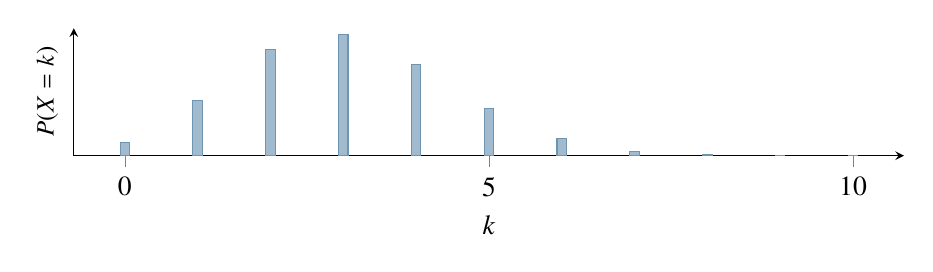
\begin{tikzpicture}
\begin{axis}[width=\textwidth,height=3.2cm,xlabel={$k$},ylabel={$P(X=k)$},
    xmin=-0.7,xmax=10.7,ymin=0,ymax=0.28,ytick=\empty,xtick={0,5,10},
    axis lines=left,ybar,bar width=3.4pt,bar shift=0pt,samples at={0,1,...,10},
    ylabel style={font=\small}]
\addplot[fill=ccBlue!45,draw=ccBlue!70]{factorial(10)/(factorial(x)*factorial(10-x))*0.3^x*0.7^(10-x)};
\end{axis}
\end{tikzpicture}
\column{0.5\textwidth}
\centering
{\small\hl{Likelihood:} fix data, $p$ varies}\\[0.4em]
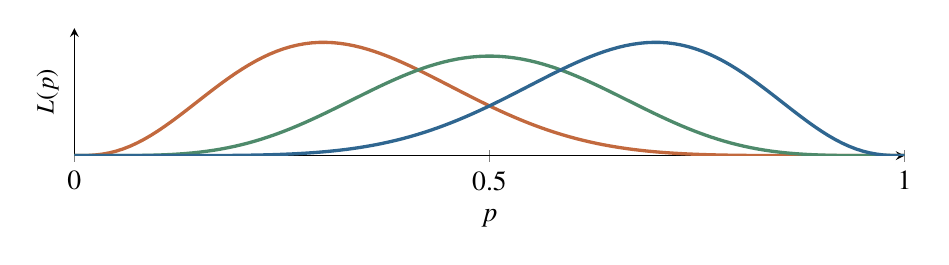
\begin{tikzpicture}
\begin{axis}[width=\textwidth,height=3.2cm,xlabel={$p$},ylabel={$L(p)$},
    xmin=0,xmax=1,ymin=0,ymax=0.0025,domain=0:1,samples=120,axis lines=left,
    xtick={0,0.5,1},ytick=\empty,ylabel style={font=\small}]
\addplot[very thick,ccTerra]{x^3*(1-x)^7};
\addplot[very thick,ccGreen]{2*x^5*(1-x)^5};
\addplot[very thick,ccBlue]{x^7*(1-x)^3};
\end{axis}
\end{tikzpicture}
\end{columns}
\centerline{\footnotesize One likelihood curve per observed count: \textcolor{ccTerra}{$X{=}3$}, \textcolor{ccGreen}{$X{=}5$}, \textcolor{ccBlue}{$X{=}7$}.}
\end{frame}


%%%%%%%%%%%%%%%%%%%%%%%%%%%%%%%%%%%%%%%%%%%%%%%%%%%%%%%%%%%%%%%%%%%%%%%%
\begin{frame}
\frametitle{Parameter estimation with maximum likelihood}
Suppose we have observed some data from a model with an unknown parameter \(\theta\). Which value of \(\theta\) makes our observed data most plausible?
\keyidea[-- Maximum likelihood]{Estimate \(\theta\) by the value with the largest likelihood:
\[ \hat\theta_{\mathrm{MLE}} = \operatorname*{arg\,max}_{\theta} L(\theta). \]}
\formula{Notation}{%
\(\operatorname*{arg\,max}_{\theta} L(\theta)\) is the \emph{value of \(\theta\)} at which \(L(\theta)\) is largest --- the \emph{arg}ument that attains the \emph{max}imum. (By contrast, \(\max_{\theta} L(\theta)\) is the largest value of \(L\) itself.)}
\end{frame}

%%%%%%%%%%%%%%%%%%%%%%%%%%%%%%%%%%%%%%%%%%%%%%%%%%%%%%%%%%%%%%%%%%%%%%%%
\begin{frame}{How the likelihood changes with the data}
\examplehead{Public transit use}
Public transit ($7$ of $10$). The data fix \emph{where} the likelihood peaks and \emph{how sharp} it is. (Rescaled; \textcolor{ccRed}{$\bullet$} marks the maximum.)
\begin{columns}[T]
\column{0.5\textwidth}
\centering
{\small More users: peak moves right}\\[0.2em]
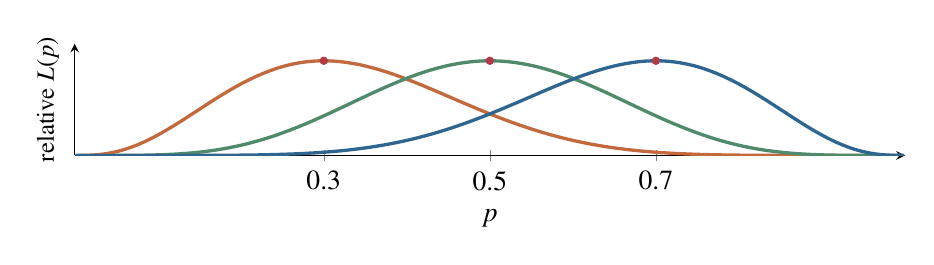
\begin{tikzpicture}
\begin{axis}[width=\textwidth,height=3.0cm,xlabel={$p$},ylabel={relative $L(p)$},
    xmin=0,xmax=1,ymin=0,ymax=1.18,domain=0.001:0.999,samples=120,axis lines=left,
    xtick={0.3,0.5,0.7},ytick=\empty,ylabel style={font=\small}]
\addplot[very thick,ccTerra]{exp(3*ln(x/0.3)+7*ln((1-x)/0.7))};
\addplot[very thick,ccGreen]{exp(5*ln(x/0.5)+5*ln((1-x)/0.5))};
\addplot[very thick,ccBlue]{exp(7*ln(x/0.7)+3*ln((1-x)/0.3))};
\addplot[only marks,mark=*,ccRed,mark size=1.3pt]coordinates{(0.3,1)(0.5,1)(0.7,1)};
\end{axis}
\end{tikzpicture}\\[0.1em]
{\scriptsize$X = $\textcolor{ccTerra}{$3$}\quad\textcolor{ccGreen}{$5$}\quad\textcolor{ccBlue}{$7$}}
\column{0.5\textwidth}
\centering
{\small More data: peak gets sharper}\\[0.2em]
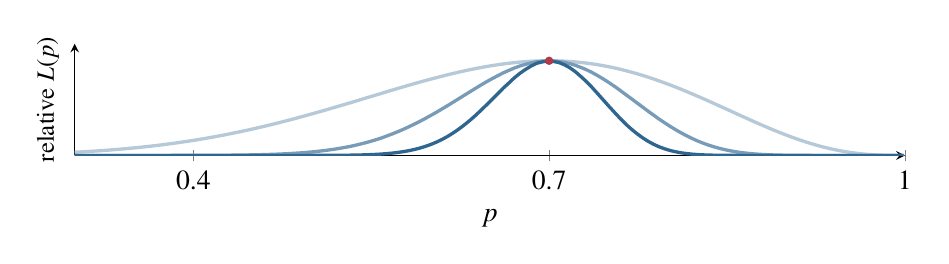
\begin{tikzpicture}
\begin{axis}[width=\textwidth,height=3.0cm,xlabel={$p$},ylabel={relative $L(p)$},
    xmin=0.3,xmax=1,ymin=0,ymax=1.18,domain=0.3:0.999,samples=150,axis lines=left,
    xtick={0.4,0.7,1},ytick=\empty,ylabel style={font=\small}]
\addplot[very thick,ccBlue!35]{exp(7*ln(x/0.7)+3*ln((1-x)/0.3))};
\addplot[very thick,ccBlue!65]{exp(28*ln(x/0.7)+12*ln((1-x)/0.3))};
\addplot[very thick,ccBlue]{exp(70*ln(x/0.7)+30*ln((1-x)/0.3))};
\addplot[only marks,mark=*,ccRed,mark size=1.3pt]coordinates{(0.7,1)};
\end{axis}
\end{tikzpicture}\\[0.1em]
{\scriptsize $n=10,\ 40,\ 100$ with $k = 0.7n$ successes (darker $=$ more data)}
\end{columns}
\end{frame}

%%%%%%%%%%%%%%%%%%%%%%%%%%%%%%%%%%%%%%%%%%%%%%%%%%%%%%%%%%%%%%%%%%%%%%%%
\begin{frame}
\frametitle{How do we find an MLE?}
\begin{enumerate}
\item Choose a probability model.
\item Write \(P(\text{observed data}\mid\theta)\).
\item Treat the data as fixed and let \(\theta\) vary.
\item Find the value of \(\theta\) where the likelihood is largest.
\end{enumerate}
\keyidea{Terms that do not involve \(\theta\) do not affect which value of \(\theta\) is best.}
\end{frame}



%%%%%%%%%%%%%%%%%%%%%%%%%%%%%%%%%%%%%%%%%%%%%%%%%%%%%%%%%%%%%%%%%%%%%%%%
\begin{frame}{Likelihood and Log-likelihood}
Suppose \(X_1,\ldots,X_n\) are independent observations from a model with parameter \(\theta\).
\formula{Likelihood and log-likelihood}{%
\begin{itemize}
\item \textbf{Likelihood:}
\[ L(\theta) = P(\text{observed data}\mid \theta) = \prod_{i=1}^{n} f(x_i\mid \theta) \]
\item \textbf{Log-likelihood:}
\[ \ell(\theta) = \log L(\theta) = \sum_{i=1}^{n} \log f(x_i\mid \theta) \]
\end{itemize}}
\end{frame}

%%%%%%%%%%%%%%%%%%%%%%%%%%%%%%%%%%%%%%%%%%%%%%%%%%%%%%%%%%%%%%%%%%%%%%%%
\begin{frame}{Likelihood and log-likelihood: same peak}
\examplehead{Public transit use}
For the transit data (7 of 10):
\begin{columns}[T]
\column{0.5\textwidth}
\centering
$L(p)=p^7(1-p)^3$ \\[.2em]
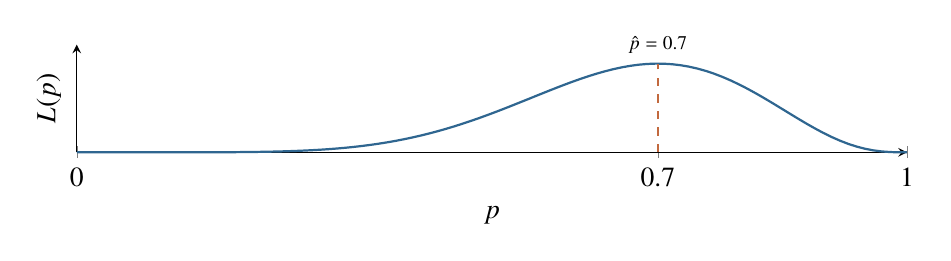
\begin{tikzpicture}
\begin{axis}[width=\textwidth,height=2.95cm,xlabel={$p$},ylabel={$L(p)$},
    xmin=0,xmax=1,ymin=0,ymax=0.0027,domain=0:1,samples=100,axis lines=left,
    xtick={0,0.7,1},ytick=\empty,clip=false]
\addplot[thick,ccBlue]{x^7*(1-x)^3};
\addplot[dashed,ccTerra]coordinates{(0.7,0)(0.7,0.002223)};
\node at (axis cs:0.7,0.002223)[anchor=south,font=\scriptsize]{$\hat p=0.7$};
\end{axis}
\end{tikzpicture}
\column{0.5\textwidth}
\centering
 $\ell(p)=7\log p+3\log(1-p)$. \\[.2em]
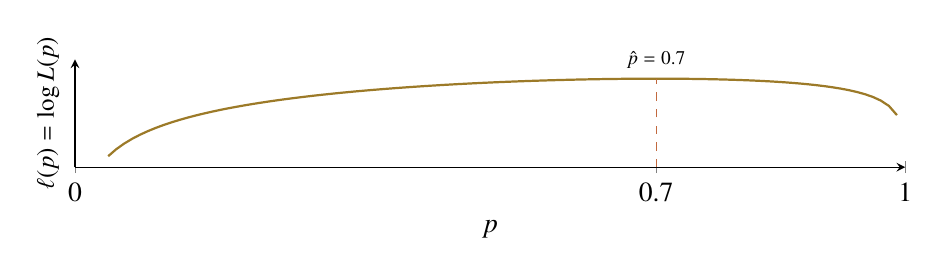
\begin{tikzpicture}
\begin{axis}[width=\textwidth,height=2.95cm,xlabel={$p$},ylabel={$\ell(p)=\log L(p)$},
    xmin=0,xmax=1,ymin=-25,ymax=-2,domain=0.04:0.99,samples=100,axis lines=left,
    xtick={0,0.7,1},ytick=\empty,ylabel style={font=\small},clip=false]
\addplot[thick,ccGold]{7*ln(x)+3*ln(1-x)};
\addplot[dashed,ccTerra]coordinates{(0.7,-25)(0.7,{7*ln(0.7)+3*ln(0.3)})};
\node at (axis cs:0.7,{7*ln(0.7)+3*ln(0.3)})[anchor=south,font=\scriptsize]{$\hat p=0.7$};
\end{axis}
\end{tikzpicture}
\end{columns}
\keyidea{Maximizing \(L(\theta)\) and maximizing \(\ell(\theta)=\log L(\theta)\) give the same answer.}
\vspace{0.2em}

\end{frame}
%%%%%%%%%%%%%%%%%%%%%%%%%%%%%%%%%%%%%%%%%%%%%%%%%%%%%%%%%%%%%%%%%%%%%%%%
\begin{frame}{Activity 2}
\activity[-- Reading likelihood plots]{%
Three studies record how many patients respond: (i) $4$ of $5$, (ii) $10$ of $20$, (iii) $16$ of $20$.
\begin{center}
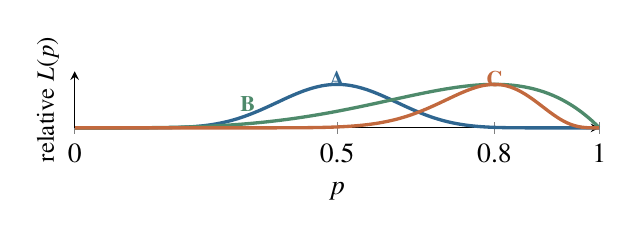
\begin{tikzpicture}
\begin{axis}[width=0.68\textwidth,height=2.3cm,xlabel={$p$},ylabel={relative $L(p)$},
    xmin=0,xmax=1,ymin=0,ymax=1.3,domain=0.001:0.999,samples=150,axis lines=left,
    xtick={0,0.5,0.8,1},ytick=\empty,ylabel style={font=\small},clip=false]
\addplot[very thick,ccBlue]{exp(10*ln(x/0.5)+10*ln((1-x)/0.5))};
\addplot[very thick,ccGreen]{exp(4*ln(x/0.8)+ln((1-x)/0.2))};
\addplot[very thick,ccTerra]{exp(16*ln(x/0.8)+4*ln((1-x)/0.2))};
\node[ccBlue,font=\footnotesize\bfseries] at (axis cs:0.5,1.12) {A};
\node[ccGreen,font=\footnotesize\bfseries] at (axis cs:0.33,0.55) {B};
\node[ccTerra,font=\footnotesize\bfseries] at (axis cs:0.8,1.12) {C};
\end{axis}
\end{tikzpicture}
\end{center}
\begin{enumerate}
\item Match each curve (A, B, C) to a study.
\item Read each MLE off the plot.
\item Which study pins down $p$ most precisely?
\end{enumerate}}
\end{frame}
%%%%%%%%%%%%%%%%%%%%%%%%%%%%%%%%%%%%

\begin{frame}{Activity 2}
\solnbox{A $\to$ (ii) $10/20$ with $\hat p=0.5$. B $\to$ (i) $4/5$: peak at $0.8$, wide. C $\to$ (iii) $16/20$: peak at $0.8$, sharp. Study (iii) pins down $p$ most precisely: more data gives a narrower peak.}
\end{frame}

%%%%%%%%%%%%%%%%%%%%%%%%%%%%%%%%%%%%

\begin{frame}{Activity 3}
\activity[-- MLE from start to finish]{%
\textbf{Worksheet Part 2:} a survey asks 12 students whether they used public transportation this week.
\begin{enumerate}
\item Choose a model and identify its parameter.
\item Count the successes and write the likelihood $L(p)$ and log-likelihood $\ell(p)$.
\item Find $\hat p_{\text{MLE}}$ and interpret it in context.
\end{enumerate}}
\end{frame}


%%%%%%%%%%%%%%%%%%%%%%%%%%%%%%%%%%%%%%%%%%%%%%%%%%%%%%%%%%%%%%%%%%%%%%%%
\begin{frame}
\frametitle{Exponential model}

The \hl{exponential distribution} models positive, right-skewed quantities:
\begin{itemize}
\item time until a website responds,
\item lifetime of a machine component,
\item size of an insurance claim.
\end{itemize}
\[
X_i\sim \text{Exponential}(\lambda), \qquad f(x_i\mid\lambda)=\lambda e^{-\lambda x_i}, \quad x_i>0.
\]
\(\lambda\) is a rate: larger \(\lambda\) means smaller values on average.
\end{frame}
%%%%%%%%%%%%%%%%%%%%%%%%%%%%%%%%%%%%%%%%%%%%%%%%%%%%%%%%%%%%%%%%%%%%%%%%
\begin{frame}{Exponential likelihood}
\workedexample[waiting times]{%
Observed waiting times (seconds): $2.1,\ 0.7,\ 1.4,\ 3.0,\ 1.8$. For independent exponential observations,
\[ L(\lambda)=\prod_{i=1}^n \lambda e^{-\lambda x_i}=\lambda^n e^{-\lambda\sum x_i}, \qquad \hat\lambda_{\mathrm{MLE}}=\tfrac{1}{\bar{x}}. \]
Here $\bar{x}=1.8$, so $\hat\lambda\approx 0.56$ events per second.}
\end{frame}
%%%%%%%%%%%%%%%%%%%%%%%%%%%%%%%%%%%%%%%%%%%%%%%%%%%%%%%%%%%%%%%%%%%%%%%%
\begin{frame}{Normal model: continuous measurements}
A Normal model is often useful for \textbf{continuous measurements} that vary around a center with roughly symmetric noise. 
\begin{itemize} 
\item Example: blood pressure reduction after treatment. 
\item Example: small measurement errors around a target value. 
\end{itemize}
Suppose we observe continuous data $x_1,x_2,\ldots,x_n$. A common model is
\[
X_i \sim N(\mu,\sigma^2).
\]
\begin{itemize}
\item $\mu$ controls the center of the distribution.
\item $\sigma^2$ controls the spread of the distribution.
\end{itemize}

\textbf{Goal:} use the observed data to estimate $\mu$ and $\sigma^2$.
\end{frame}

%%%%%%%%%%%%%%%%%%%%%%%%%%%%%%%%%%%%%%%%%%%%%%%%%%%%%%%%%%%%%%%%%%%%%%%%
\begin{frame}{A second running example}
\examplehead{Repeated measurements}
\textbf{Question.} A lab measures the same specimen five times. What is the true value, and how variable is the measurement process?
\medskip

\textbf{Data.} The measurements are $2,\ 4,\ 5,\ 6,\ 8$ (sample mean $\bar x = 5$).
\medskip

\textbf{Model.} $X_i \sim N(\mu,\sigma^2)$, where $\mu$ is the true value and $\sigma$ describes the measurement variability.
\end{frame}

%%%%%%%%%%%%%%%%%%%%%%%%%%%%%%%%%%%%%%%%%%%%%%%%%%%%%%%%%%%%%%%%%%%%%%%%
\begin{frame}{Fitting a normal: which $\mu$ and $\sigma$?}
\examplehead{Repeated measurements}
Five measurements ($\bar x=5$). Each candidate $(\mu,\sigma)$ gives a normal curve. Which curve fits the data best?
\begin{center}
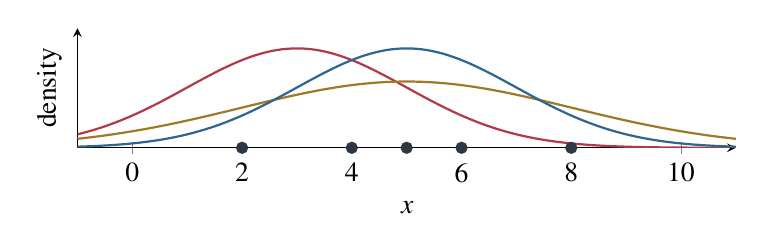
\begin{tikzpicture}
\begin{axis}[width=0.82\textwidth,height=3.1cm,xlabel={$x$},ylabel={density},
    xmin=-1,xmax=11,ymin=0,ymax=0.24,domain=-1:11,samples=120,axis lines=left,ytick=\empty]
\addplot[thick,ccRed]{1/(2*sqrt(2*pi))*exp(-(x-3)^2/(2*4))};
\addplot[thick,ccGold]{1/(3*sqrt(2*pi))*exp(-(x-5)^2/(2*9))};
\addplot[thick,ccBlue]{1/(2*sqrt(2*pi))*exp(-(x-5)^2/(2*4))};
\addplot[only marks,mark=*,mark size=2pt,color=ccSlate]coordinates{(2,0)(4,0)(5,0)(6,0)(8,0)};
\end{axis}
\end{tikzpicture}\\[0.1em]
{\scriptsize\textcolor{ccRed}{$\mu=3,\ \sigma=2$: off-center}\qquad\textcolor{ccGold}{$\mu=5,\ \sigma=3$: too wide}\qquad\textcolor{ccBlue}{$\mu=5,\ \sigma=2$: best fit}}
\end{center}
\vspace{-0.2em}
The best fit (maximum likelihood) parameters center on the data ($\mu=\bar x=5$) with spread matching the scatter. 
\end{frame}
%%%%%%%%%%%%%%%%%%%%%%%%%%%%%%%%%%%%%%%%%%%%%%%%%%%%%%%%%%%%%%%%%%%%%%%%
\begin{frame}{Likelihood for a normal model}
If
\[
X_i \sim N(\mu,\sigma^2),
\]
then the density of one observation is
\[
f(x_{i} \mid \mu, \sigma^{2}) 
=
\frac{1}{\sqrt{2\pi\sigma^2}}
\exp\left(
-\frac{(x_i-\mu)^2}{2\sigma^2}
\right).
\]
For independent observations, the likelihood is
\begin{align*}
L(\mu, \sigma^{2}) 
&=
\prod_{i=1}^{n} f(x_{i} \mid \mu, \sigma^{2}) \\
&=
\prod_{i=1}^{n}
\frac{1}{\sqrt{2\pi\sigma^2}}
\exp\left(
-\frac{(x_i-\mu)^2}{2\sigma^2}
\right).
\end{align*}
\end{frame}

%%%%%%%%%%%%%%%%%%%%%%%%%%%%%%%%%%%%%%%%%%%%%%%%%%%%%%%%%%%%%%%%%%%%%%%%
\begin{frame}{The likelihood is a surface}
\examplehead{Repeated measurements}
With two unknowns, the likelihood $L(\mu,\sigma)$ is a \hl{surface}; its highest point sits above the maximum likelihood estimates. (Data $2,4,5,6,8$; height rescaled so the peak is $1$.)
\begin{center}
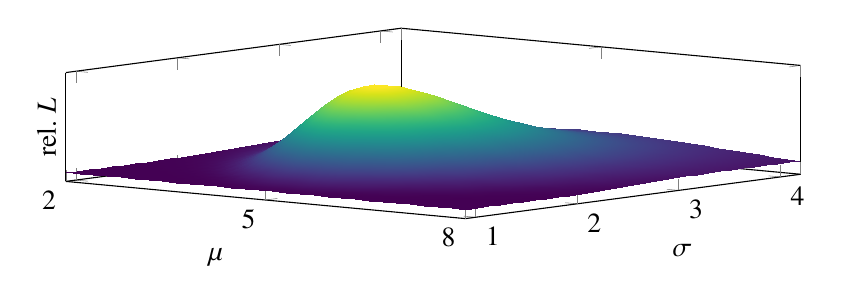
\begin{tikzpicture}
\begin{axis}[width=0.9\textwidth,height=4.0cm,view={40}{28},
    xlabel={$\mu$},ylabel={$\sigma$},zlabel={rel.\ $L$},
    domain=2:8,y domain=0.9:4.2,samples=30,samples y=30,
    colormap/viridis,ztick=\empty,xtick={2,5,8},ytick={1,2,3,4}]
\addplot3[surf,shader=interp]{exp(-5*ln(y/2)-5*((x-5)^2+4)/(2*y^2)+2.5)};
\end{axis}
\end{tikzpicture}
\end{center}
\vspace{-0.2em}
\centerline{The peak is at $\hat\mu=\bar x=5$ and $\hat\sigma=2$.}
\end{frame}

%%%%%%%%%%%%%%%%%%%%%%%%%%%%%%%%%%%%%%%%%%%%%%%%%%%%%%%%%%%%%%%%%%%%%%%%
\begin{frame}{The data locate the peak}
\examplehead{Repeated measurements}
Change the data and the surface --- and its peak --- moves. Here the peak tracks the sample mean $\bar x$. (Top-down view; brighter $=$ higher likelihood.)
\vspace{0.1em}
\begin{columns}[T]
\column{0.5\textwidth}
\centering
{\small Data $2,4,5,6,8$:\ $\bar x=5$}\\[0.2em]
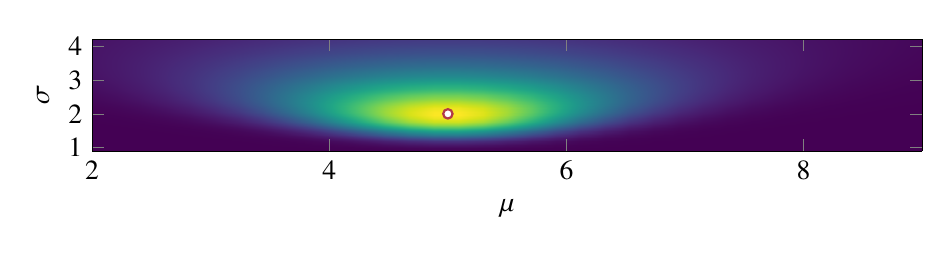
\begin{tikzpicture}
\begin{axis}[width=\textwidth,height=3.0cm,view={0}{90},
    xlabel={$\mu$},ylabel={$\sigma$},domain=2:9,y domain=0.9:4.2,
    samples=35,samples y=35,colormap/viridis,enlargelimits=false,axis on top,
    xtick={2,4,6,8},ytick={1,2,3,4}]
\addplot3[surf,shader=interp]{exp(-5*ln(y/2)-5*((x-5)^2+4)/(2*y^2)+2.5)};
\node[circle,fill=white,draw=ccRed,line width=0.8pt,inner sep=1.2pt]at(axis cs:5,2,1){};
\end{axis}
\end{tikzpicture}
\column{0.5\textwidth}
\centering
{\small Each value $+1.5$:\ $\bar x=6.5$}\\[0.2em]
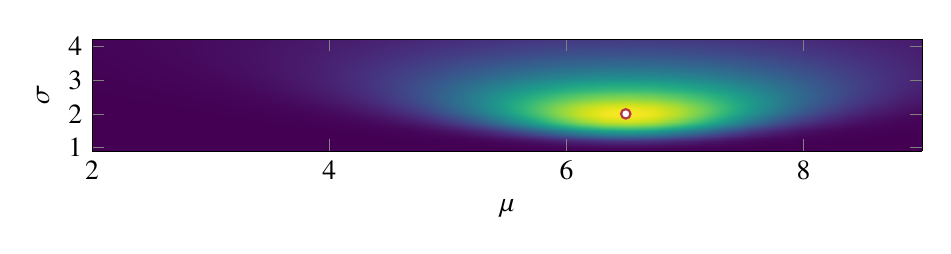
\begin{tikzpicture}
\begin{axis}[width=\textwidth,height=3.0cm,view={0}{90},
    xlabel={$\mu$},ylabel={$\sigma$},domain=2:9,y domain=0.9:4.2,
    samples=35,samples y=35,colormap/viridis,enlargelimits=false,axis on top,
    xtick={2,4,6,8},ytick={1,2,3,4}]
\addplot3[surf,shader=interp]{exp(-5*ln(y/2)-5*((x-6.5)^2+4)/(2*y^2)+2.5)};
\node[circle,fill=white,draw=ccRed,line width=0.8pt,inner sep=1.2pt]at(axis cs:6.5,2,1){};
\end{axis}
\end{tikzpicture}
\end{columns}
\vspace{0.1em}
The spread is unchanged, so $\hat\sigma=2$ in both; only $\hat\mu$ shifts (from $5$ to $6.5$).
\end{frame}
%%%%%%%%%%%%%%%%%%%%%%%%%%%%%%%%%%%%%%%%%%%%%%%%%%%%%%%%%%%%%%%%%%%%%%%%
\begin{frame}{Log-likelihood for a normal model}
Taking logs gives
\[
-\frac{n}{2}\log(2\pi)
-\frac{n}{2}\log(\sigma^2)
-\frac{1}{2\sigma^2}
\sum_{i=1}^{n}(x_i-\mu)^2.
\]
\begin{itemize}
\item Maximizing the log-likelihood over $\mu$ is the same as minimizing
\[
\sum_{i=1}^{n}(x_i-\mu)^2.
\]
\item This is the sum of squared distances from the data values to $\mu$.

\item The value of $\mu$ that minimizes this quantity is the sample mean.
\end{itemize}
\end{frame}
%%%%%%%%%%%%%%%%%%%%%%%%%%%%%%%%%%%%%%%%%%%%%%%%%%%%%%%%%%%%%%%%%%%%%%%%
\begin{frame}{Maximum likelihood estimates for a normal model}
\formula{Normal MLEs}{%
\[ \widehat{\mu}_{\mathrm{MLE}} = \bar{x} = \frac{1}{n}\sum_{i=1}^{n}x_i, \qquad
   \widehat{\sigma}^{2}_{\mathrm{MLE}} = \frac{1}{n}\sum_{i=1}^{n}(x_i-\bar{x})^2. \]}
\begin{itemize}
\item \(\widehat{\mu}_{\mathrm{MLE}}\) is the sample mean.
\item \(\widehat{\sigma}^{2}_{\mathrm{MLE}}\) is the average squared distance from the sample mean.
\item The MLE of the variance uses denominator \(n\), not \(n-1\).
\end{itemize}
\end{frame}
%%%%%%%%%%%%%%%%%%%%%%%%%%%%%%%%%%%%

\begin{frame}{Activity 4}
\activity[-- a normal model]{%
\textbf{Worksheet Part 3:} four webpage loading times are recorded, with $X_i\sim N(\mu,\sigma^2)$.
\begin{enumerate}
\item Compute $\hat\mu_{\text{MLE}}=\bar{x}$.
\item Compute $\hat\sigma^2_{\text{MLE}}$ (denominator $n$, not $n-1$).
\item Say in one sentence what $\sigma^2$ measures.
\end{enumerate}}
\end{frame}

%%%%%%%%%%%%%%%%%%%%%%%%%%%%%%%%%%%%%%%%%%%%%%%%%%%%%%%%%%%%%%%%%%%%%%%%
\begin{frame}
\frametitle{Summary: MLE for simple models}

\begin{center}
\small
\begin{tabular}{p{0.25\textwidth}p{0.4\textwidth}p{0.2\textwidth}}
\hline
\textbf{Model} & \textbf{Observed data} & \textbf{MLE}\\
\hline
Bernoulli\((p)\) & sequence of 0s and 1s & \(\hat p=\) sample proportion\\[0.3em]
Binomial\((n,p)\) & successes out of fixed \(n\) & \(\hat p=x/n\)\\[0.3em]
Exponential\((\lambda)\) & positive values & \(\hat\lambda=1/\bar{x}\)\\[0.3em]
Normal\((\mu,\sigma^2)\) & continuous measurements & \(\hat\mu=\bar{x}\), \(\hat\sigma^2=\frac{1}{n}\sum(x_i-\bar{x})^2\)\\
\hline
\end{tabular}
\end{center}
\end{frame}
%%%%%%%%%%%%%%%%%%%%%%%%%%%%%%%%%%%%%%%%%%%%%%%%%%%%%%%%%%%%%%%%%%%%%%%%
% End document

\end{document}